\subsection{Basic Algorithm}

The basic system will be to connect interested peers with one another via a DHT that stores peers lists, and the peers themselves will become part of the DHT.  They will store only peer information on the DHT, not blocks themselves.
% why is in the other one...less intrusive.

In our protocol, a peer first tries to download the file from an origin web server.  If at some point one of the following conditions occurs, the download switches to a peer-to-peer swarming download:
\begin{enumerate}
\item First, the client waits a maximum number of seconds $T$ after the start of a normal HTTP download to receive the first byte of data.  If $T$ seconds passes without receiving any data, it transitions to P2P download.  This allows the system to decide quickly whether the origin server is over-burdened and switch to peer-to-peer if needed.   
\item Once the client receives some data from the server, it monitors whether the receive rate falls below a certain fixed threshold $R$ bytes per second over a window of of the last $W$ seconds.  If the receive rate ever drops below $R$, the client switches to peer-to-peer delivery.  This is to accomodate for servers with slow connections or file downloads that become slower mid-download.
\end{enumerate}

Once a client decides to switch to peer-to-peer downloading, it may need to first lookup meta-data about the file (for example, the size).  To do so the client  calculates a hash value for the URI being download, and looks that up as a $key$ value in the DHT to retrieve meta-data.  After this, peers randomly choose $b$ blocks of the file to download, and retrieve lists of peers who have those blocks by hashing the URI and block number.  The peer chooses one peer per block list and downloads from that peer, for several blocks at the same time.  After downloading a block, it then adds itself to the list of peers willing to share that block (see Fig. \ref{fig:download_all_steps}).  While it is attempting to enumerate peers for a block, it attempts to download the block from the origin server, as well, to not have wasted any time if no peers are found.  If a peer downloads a file whose meta-data is not listed in the DHT, it will also add that meta-data after downloading it (for instance, the very first time a peer downloads a file, it will notice its absence on the DHT and update it accordingly).  To combat the ``slow last block'' problem,  peers download the last block from several peers simultaneously, similar to BitTorrent \footnote{In reality, we download from $b$ peers at a time, including for the last blocks, i.e. if you have $b$ set to 10 and have 5 blocks left, each will be downloaded by 2 peers simultaneously, and so on down to the last block being downloaded by all $b$ connections redundantly.}.

\begin{figure*}
  \begin{center}
    \subfigure[Peer downloads list of blocks]{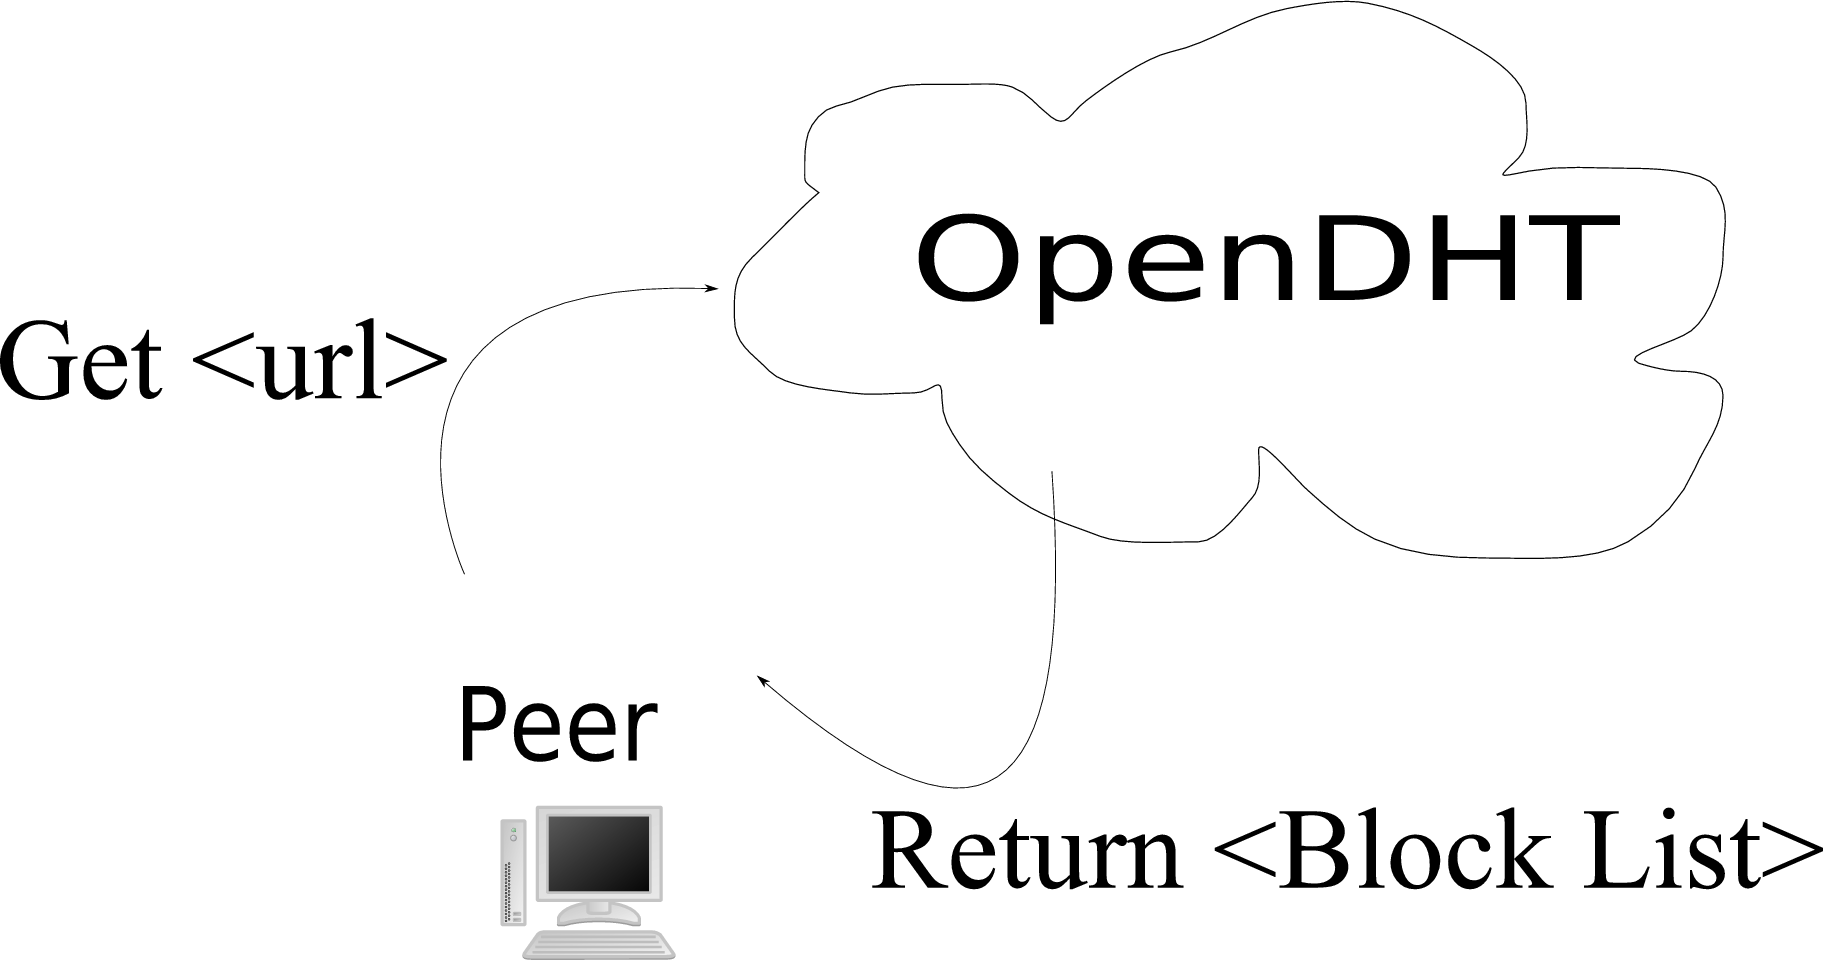
\includegraphics[width=7cm]{description_pics/peer_step_1.png}}
    \subfigure[Peer downloads a list of peers which have a block]{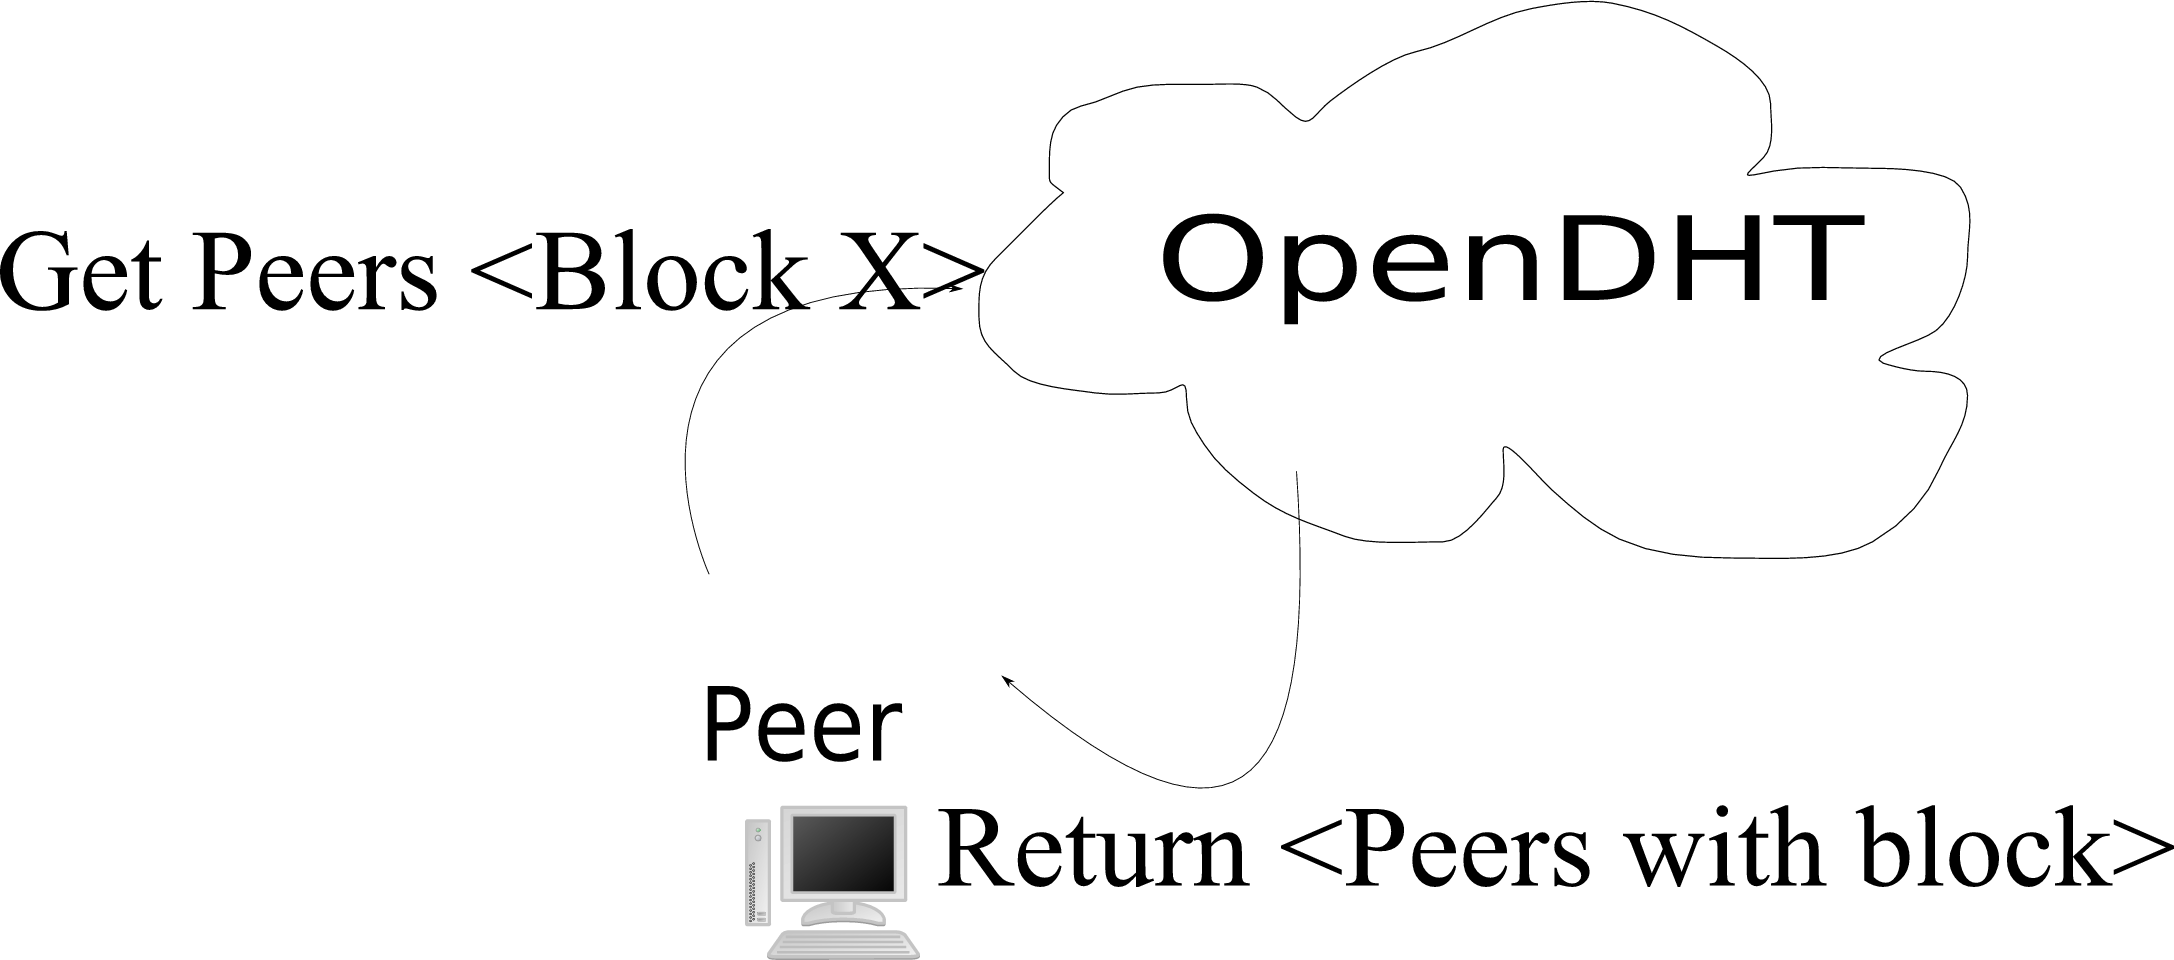
\includegraphics[width=7cm]{description_pics/peer_step_2.png}}
    \subfigure[Peer adds itself to list of peers who have that block]{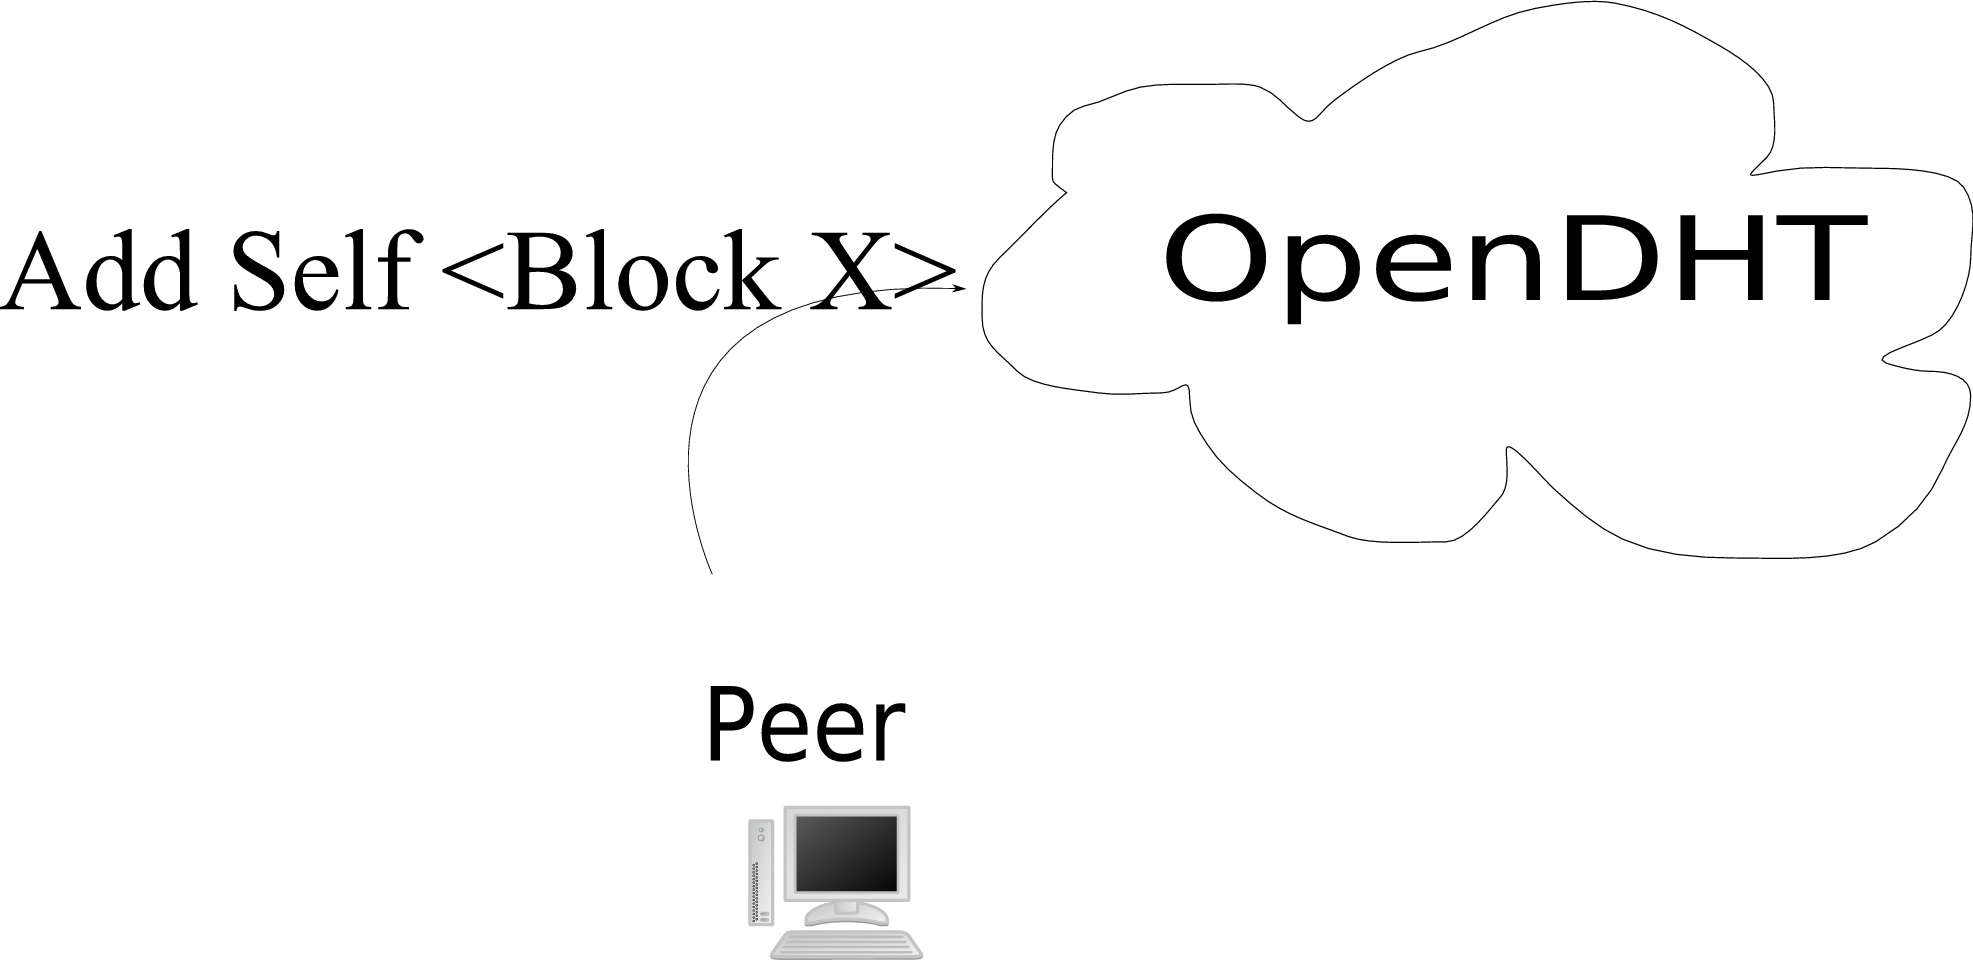
\includegraphics[width=7cm]{description_pics/peer_step_3.png}}
    \caption{Steps to accomplish a peer-to-peer-web download.}
    \label{fig:download_all_steps}
  \end{center}
\end{figure*}


